\documentclass[abstracton,11pt]{scrartcl}

%personel data
\title{Lagrange-Formulierung \\ und \\ Elektrodynamik via Differentialformen I}
\author{Eugen Dizer \& Mathieu Kaltschmidt}
\date{09. April 2018}

%math and theorems
\usepackage{amsmath}
\usepackage{ntheorem}
\usepackage{amssymb}


%language settings and microtype
\usepackage{fontspec} 
\setmainfont{Palatino}
\setsansfont{Optima}
\setmonofont[Scale=MatchLowercase]{Menlo}

\usepackage{polyglossia}
\setmainlanguage{german}
\setotherlanguages{english}
\usepackage{microtype}

%useful packages
\usepackage{geometry}
\usepackage{xcolor}
\usepackage{graphicx}
\usepackage{float}
\usepackage{fancyhdr}
\usepackage{csquotes}
\usepackage{blindtext}
\usepackage{todonotes}
\usepackage{physics}


%geometry
\geometry{
	width=150mm,
}

%color settings
\definecolor{myred}{RGB}{196,19,47} 
\definecolor{myblue}{RGB}{0,139,139}


%for empty pages at the beginning of the document
\def\blankpage{%
	\clearpage%
	\thispagestyle{empty}
	\addtocounter{page}{-1}
	\null%
	\clearpage}

% Page layout for beginning of chapter
\fancypagestyle{plain}{%
	\fancyhf{}  % clear all header and footer fields 
	\fancyfoot[C]{- \thepage\hspace{3pt}-} 
	\renewcommand{\headrulewidth}{0pt}
	\renewcommand{\footrulewidth}{0pt}}

%page layout for the other pages
\makeatletter
\pagestyle{fancy}
\fancyhf{}
\fancyhead[L]{\textit{\leftmark}}
\fancyfoot[C]{- \thepage\hspace{3pt}-}
\renewcommand{\headrulewidth}{0.2pt}
\renewcommand{\footrulewidth}{0pt}
\makeatother

% titles and stuff
\setkomafont{section}{\normalfont\bfseries\Large}
\setkomafont{subsection}{\normalfont\bfseries\large}
\setkomafont{subsubsection}{\normalfont\bfseries\normalsize}

%nice boxes
\usepackage[many]{tcolorbox}    
\newtcolorbox{mybox}[1]{%
	tikznode boxed title,
	enhanced,
	arc=0mm,
	interior style={white},
	attach boxed title to top center= {yshift=-\tcboxedtitleheight/2},
	fonttitle=\large\bfseries,
	colbacktitle=white,coltitle=black,
	boxed title style={size=normal,colframe=white,boxrule=0pt},
	title={#1}}

% nice fracs
\usepackage{xfrac}

%parindent
\setlength{\parindent}{0pt}

%bibliography
\usepackage[
style=numeric-comp,
backend=biber,
isbn=false,
date=year,
url=false,
doi=false
]{biblatex}
\addbibresource{bibliography/electrodynamics-bib.bib}


%appendix
\usepackage[toc,page]{appendix}

%always use heperref at the end of the preamble!
\usepackage[colorlinks=True]{hyperref}
\hypersetup{allcolors=myred}

%new commands 
\newcommand{\lagr}{\mathcal{L}}
\newcommand{\w}{\wedge}
\newcommand{\fu}{F^{\mu \nu}}
\newcommand{\fd}{F_{\mu \nu}}
\newcommand{\dct}{\partial_{ct}}
\newcommand{\hodge}{\text{*dF}}


\begin{document}	
%Titel und Vorwort
\begin{center}

	\makeatletter
	\thispagestyle{plain}
	\LARGE\textbf{\@title} \\
	\vspace{2mm}
	\large\bfseries{\@author} \\
	\normalfont
	\vspace{2mm}
	\large{\@date} \\
	\vspace{2mm}
	\large{Institut für Theoretische Physik \\
		Universität Heidelberg} \\
	\makeatother
\end{center}

\normalsize

Dieser Vortrag entstand im Rahmen des Seminars "\textit{Klassische Elektrodynamik}", organisiert von Prof. Weigand am Institut für Theoretische Physik der Universität Heidelberg im Sommersemester 2018. \\
Ziel des Vortrages ist es, eine Formulierung der Elektrodynamik in Differentialformen zu motivieren und damit eine alternative Formulierung der Maxwell-Gleichungen einzuführen. Es werden die mathematischen und physikalischen Grundlagen für das Verständnis der modernen Eichtheorien besprochen und die Elektrodynamik als klassische Feldtheorie vorgestellt. \\
Zu Beginn soll die Lagrange-Formulierung der kovarianten Elektrodynamik thematisiert werden, um sie am Ende in der Sprache der Differentialformen zu formulieren.

	
% Inhalt

% erster Teil
\section{Lagrange-Formulierung der Elektrodynamik}
Das Hamilton'sche Extremalprinzip ist in vielen Anwendungen sehr erfolgreich. Es charakterisiert physikalisch realisierbare Bahnen unter allen denkbaren Bahnen als diejenigen, die kritische Elemente des Wirkungsintegrals sind. Die Lagrangefunktion dient nicht nur zur rationalen Herleitung der Bewegungsgleichungen, sondern ist auch ein wichtiges Hilfsmittel zur Bestimmung von Erhaltungsgrößen.
Wir werden diese mächtige Methode auf die Elektrodynamik anwenden und sie auf überabzählbar viele Freiheitsgrade erweitern.

\subsection{Lagrangedichte für eine Feldtheorie}
In der klassischen Mechanik hatten wir es immer mit endlich vielen Freiheitsgraden zu tun. Bei der klassischen Feldtheorie stellen wir uns den Raum als gitterartig verbundene Raumpunkte vor, die jeweils mit ihren Nachbarn wechselwirken können. Im Kontinuumslimit haben wir unendlich viele Raumpunkte und benötigen eine neue Beschreibungsweise. \\
An die Stelle der verallgemeinerten Koordinaten treten nun die \textbf{Felder} $\varphi^{(i)}$ und die Lagrangefunktion wird durch die \textbf{Lagrangedichte} \  $\text{L}=\iiint \dd[3]{x}  \lagr$ \ ersetzt. \\
Das Wirkungsintegral ist nun $\text{I}=\int_{t_1}^{t_2} \dd{t} \iiint \dd[3]{x}  \lagr = \int \dd[4]{x} \lagr$. \\
Die Bewegungsgleichungen erhalten wir aus dem Hamiltonschen Prinzip und nehmen dazu an, dass die Variation der Felder auf den Hyperflächen $t=t_1$ und $t=t_2$ verschwindet:
\begin{align*}
0 = \delta I &= \int \dd[4]{x} \left( \dphi \delta\varphi^{(i)} + \ddphi \delta(\partial_{\mu}\varphi^{(i)}) \right) \\
 				 &= \int \dd[4]{x} \left(\dphi - \partial_{\mu} \ddphi \right) \delta\varphi^{(i)}
\end{align*}
Wir erhalten daraus:
\begin{mybox}{Euler-Lagrange-Gleichung}

\begin{align}
0=\dphi - \partial_{\mu} \ddphi
\end{align}

\end{mybox}

\subsection{Lagrangedichte für das Maxwell-Feld}
Wir wollen $\lagr$ \ so wählen, dass sie ein Skalar ist, von den Feldern sowie deren Ableitungen abhängt, Strom/Ladung als Quelle hat und die Maxwell-Gleichungen als Bewegungsgleichungen liefert:
\begin{align}
\partial_{\mu}\fu = j^{\nu} \qquad  \Longleftrightarrow \qquad \Box A^{\nu} - \partial^{\nu}(\partial_{\mu}A^{\mu}) = j^{\nu}
\end{align}
Da wir als Bewegungsgleichungen Differentialgleichungen 2. Ordnung erwarten, bietet es sich an, das 4er-Feld $A^{\mu}$ wie folgt anzusetzen:
\begin{align*}
\lagr = \text{a} \cdot \partial_{\mu}A^{\nu}\partial^{\mu}A_{\nu} + \text{b} \cdot \partial_{\mu}A^{\nu}\partial_{\nu}A^{\mu} + \text{c} \cdot (\partial_{\mu}A^{\mu})^2 + \text{d} \cdot A_{\mu}A^{\mu} + \text{e} \cdot A_{\mu}j^{\mu}
\end{align*}
Setzt man dies in (1) ein und wählt die Koeffizienten so, dass (2) herauskommt, findet man:
\begin{align*}
\lagr = -\frac{1}{4} \fd \fu - j_{\mu}A^{\mu} + \frac{\text{c}}{2} \underbrace{\left[ (\partial_{\mu}A^{\mu})^2 - \partial_{\mu}A^{\nu}\partial_{\nu}A^{\mu} \right]}_{= \partial_{\mu}(A^{\mu}\partial_{\varrho}A^{\varrho}-A_{\nu}\partial^{\nu}A^{\mu})}
\end{align*}
Da der letzte Term sich als Divergenz schreiben lässt, ist er nur ein Randterm und verschwindet bei der Variation. Er ändert somit nichts an den Bewegungsgleichungen! \\ 
Es folgt also:
\begin{mybox}{Lagrangedichte}
\begin{align}
\lagr = -\frac{1}{4} \fd \fu - j_{\mu}A^{\mu}
\end{align}
\end{mybox}
\phantom{.} \\
Die Lagrangedichte hat demnach die richtige Dimension $\left[\sfrac{\text{Energie}}{\text{Volumen}}\right]$ wobei der erste Term einer "kinetischen Energie" und der Zweite einer "potentiellen Energie" entspricht. \\

Andererseits kann man die Lagrangedichte auch ohne Kenntnis der Maxwell-Gleichungen herleiten. \\
Wir wissen, dass die Elektrodynamik eine relativistische Theorie ist und die Bewegungsgleichungen daher invariant unter Lorentz-Transformationen sein sollten. Außerdem gilt das Superpositionsprinzip, d.h. Summen von Lösungen der Bewegungsgleichungen sind wieder Lösungen. deshalb sollten die Bewegungsgleichungen linear sein, der Lagrangian also höchstens quadratisch in den Ableitungen der Feldkomponenten sein. \\ 
Zuletzt sollen die Bewegungsgleichungen eichinvariant sein.
Aus den obigen Überlegungen ergeben sich folgende Forderungen an den Lagrangian: \\
\begin{enumerate}
	\item Lorentzinvarianz
	\item Eichinvarianz 
	\item  Höchstens quadratisch in den Ableitungen
\end{enumerate}

Aus der ersten Forderung folgt, dass die Lagrangedichte ein Lorentz-Skalar sein muss. Aus der Eichinvarianz folgt, dass die Lagrangedichte $\fd$ oder sein Pendant $\star \fd$ enthalten kann, denn unter einer Eichtransformation $A^{\mu} \rightarrow A^{\mu} + \partial^{\mu} \phi$ ändert sich der Feldstärketensor nicht:

\begin{align}
\fd ' = \partial_{\mu} \left( A^{\nu} + \partial_{\nu} \phi \right) - \partial_{\nu} \left( A^{\mu} + \partial_{\mu} \phi \right) = \partial_{\mu}  A^{\nu} - \partial_{\nu} A^{\mu} = \fd.
\end{align}

Da $\fd$ spurfrei ist, sind die ersten Skalare, die nur quadratisch von den Ableitungen abhängen:

\begin{align}
\fd \fu &= - \left( \star \fd \right) \left( \star \fu \right) = 2 \left( \vec{B}^2 - \vec{E}^2 \right) \\
\left( \star \fd \right) \fu &= 4 \vec{B} \cdot \vec{E}
\end{align}

Betrachtet man diese beiden Skalare ausführlicher, fällt auf, dass der Zweite sein Vorzeichen unter Raumspiegelung ändert. Solche paritätsverletzenden Effekte wurden bisher nicht beobachtet, weshalb dieser als Kandidat rausfällt. Da wir höchstens quadratische Abhängigkeiten in den Ableitungen zulassen wollen, haben wir diese mit $\fd \fu$ gefunden. Mehr Kombinationen, sodass es eichinvariant bleibt, gibt es nicht. Betrachten wir also noch die reinen Feldanteile: \\

Am einfachsten wäre $A_{\mu} A^{\mu}$. Dies entspricht aber einem Massenterm, der dazu führen würde, dass die Felder schneller als $\sfrac{1}/{r{}$ abfallen würden. Deshalb bleibt noch der Lorentz-Skalar $j_{\mu} A^{\mu}$, der mit der Kontinuitätsgleichung $\partial_{\mu} j^{\mu} = 0$ eichinvariant ist. Da es die Symmetrie der Natur verletzen würde, dürfen die Raumzeitkoordinten $x^{\mu}$ nicht explizit vorkommen. \\

Die drei Forderungen fixieren die Lagrangedichte demnach auf $\lagr = a \cdot \fd \fu + b \cdot j_{\mu} A^{\mu}$. 

	\subsection{Eichtransformationen und Eichinvarianz}
Die Eichtransformation $A_{\mu} \rightarrow A'_{\mu} = A_{\mu} - \partial_{\mu}\phi$ \ ändert die Lagrangedichte im Allgemeinen:
\begin{align}
\lagr'(A'_{\tau},\partial_{\tau}A'_{\tau}) = \lagr(A_{\tau},\partial_{\tau}A_{\tau})+ j^{\mu}\partial_{\mu}\phi
\end{align}
Da die Kontinuitätsgleichung $\partial_{\mu}j^{\mu}=0$ gilt, kann man $j^{\mu}\partial_{\mu}\phi$ durch $\partial_{\mu}(j^{\mu}\phi)$ ersetzen.
Dies lässt sich wieder als Divergenz auffassen und hat deshalb keinen Einfluss auf die Bewegungsgleichungen:

\begin{align*}
\text{Ladungserhaltung} \qquad \longleftrightarrow \qquad \text{Eichinvarianz}
\end{align*}
\\
Besonders interessant sind Translationen $x \rightarrow x + \varepsilon \cdot a$: 
\begin{align*}
\varphi^{(i)}(x + \varepsilon \cdot a) &= \varphi^{(i)}(x) + \overbrace{\varepsilon\cdot a^{\mu}\partial_{\mu}\varphi^{(i)}(x)}^{\delta\varphi^{(i)}} \\
\partial_{\mu}\varphi^{(i)}(x + \varepsilon \cdot a) &= \partial_{\mu}\varphi^{(i)}(x) + \underbrace{\varepsilon\cdot\left(a^{\nu}\partial_{\nu}\partial_{\mu}\varphi^{(i)}(x) + \partial_{\mu}a^{\nu}\partial_{\nu}\varphi^{(i)}(x)\right)}_{\delta(\partial_{\mu}\varphi^{(i)})} 
\end{align*}
Es wurde hierbei angenommen, dass die Ortsabhängigkeit nur in den Feldern steckt. \\
Wir erhalten:
\begin{align*}
\delta \mathcal{S} &= \int \dd[4]{x} \left( \dphi \ \varepsilon\cdot a^{\mu}\partial_{\mu}\varphi^{(i)} + \ddphi \ \varepsilon\cdot\left(a^{\nu}\partial_{\nu}\partial_{\mu}\varphi^{(i)}+\partial_{\mu}a^{\nu}\partial_{\nu}\varphi^{(i)}\right) \right) \\
&= \int \dd[4]{x} \left( \partial_{\nu}\lagr - \partial_{\mu} \left[\ddphi \partial_{\nu}\varphi^{(i)}\right] \right) \varepsilon\cdot a^{\nu}
\end{align*}
Damit erhalten wir:
\begin{mybox}{Energie-Impuls-Tensor}
\begin{align}
\partial_{\mu}\underbrace{\left[ \ddphi \partial^{\nu}\varphi^{(i)} - g^{\mu \nu}\lagr \right]}_{ = \eitens} = 0
\end{align}
\end{mybox}

Für das elektromagnetische Feld $\lagr = -\frac{1}{4} \fd \fu - j_{\mu}A^{\mu}$ folgt:

\begin{align}
\eitens = - \fu j^{\nu}A_{\sigma}+g^{\mu\nu}\left( \frac{1}{4} F_{\sigma\tau}F^{\sigma\tau}+j_{\mu}A^{\mu}\right)
\end{align}

In dieser Fom ist der Energie-Impuls-Tensor aber nicht eichinvariant, denn unter der Transformation $A^{\mu} \ \rightarrow \ A^{\mu} + \partial^{\mu}\phi$ folgt:

\begin{align}
\eitens \quad \rightarrow \quad \eitens + g^{\mu\nu}j_{\tau}\partial^{\tau}\phi-F^{\mu\sigma}\partial^{\nu}\partial_{\sigma}\phi = \eitens + \partial_{\sigma}(g^{\mu\nu}j^{\sigma}\phi - F^{\mu\sigma}j^{\nu}\phi) - j^{\mu}\partial^{\nu}\phi
\end{align}

Wir wollen einen Ausdruck für $\eitens$ finden, der eichinvariant und symmetrisch ist. \\
Dazu bemerken wir, dass zur Lagrangedichte eine Divergenz addiert werden kann ohne die Bewegungsgleichungen zu ändern. Also hat der Energie-Impuls-Tensor eine gewisse Beliebigkeit, die wir ausnutzen können. \\
Der Energiestrom bleibt unverändert unter einer Transformation $\eitens \ \rightarrow \ \eitens+ \grad{\eitens}$ mit: 

\begin{enumerate}
\item[(i)] $\partial_{\mu}\grad{\eitens}=0$ \qquad (erfüllt Erhaltungssatz)
\item[(ii)] $ \int \dd[3]{x} \grad{T^{00}}$ \qquad \ (trägt nicht zur Gesamtenergie bei)
\end{enumerate}

Obiger Zusatzterm nach der Eichung motiviert $\grad{\eitens}=\partial_{\sigma}(F^{\mu\sigma}A^{\nu})$ und erfüllt die Bedingungen. \\
Setzen wir also:

\begin{align}
\eitens = -F^{\mu\sigma}\partial^{\nu}A_{\sigma} + g^{\mu\nu}\left( \frac{1}{4}F_{\sigma\tau}F^{\sigma\tau} + j_{\tau}A^{\tau} \right) + \partial_{\sigma} \left(F^{\mu\sigma}A^{\nu} \right)
\end{align}

und schreiben mit der Maxwell-Gleichung $\partial_{\sigma}F^{\mu\sigma}=-j^{\mu}$ den neuen Ausdruck:

\begin{align}
\eitens = F^{\mu\varrho}F_{\varrho}^{\phantom{\varrho}\nu} + \frac{1}{4}g^{\mu\nu}F_{\sigma\tau}F^{\sigma\tau} + g^{\mu\nu}j_{\sigma}A^{\sigma} - j^{\mu}A^{\nu}
\end{align}

Damit gilt $\partial_{\mu}\eitens = A_{\varrho}\partial^{\nu}j^{\varrho}$. \\
Für den rein elektromagnetischen Anteil $\eitens_0 = \fu F_{\sigma}^{\phantom{\sigma}\nu} + \frac{1}{4}g^{\mu\nu}F_{\sigma\tau}F^{\sigma\tau}$ folgt dann: $\partial_{\mu}\eitens_0=j_{\varrho}F^{\varrho\nu}$. \\
\vspace{1pt} \\
In Abwesenheit von äußeren Quellen ist der Energie-Impuls-Tensor \textbf{eichinvariant}, \textbf{erhalten}, \textbf{symmetrisch} und \textbf{spurfrei}.


% zweiter Teil	
\newpage
\section{Elektrodynamik in Differentialformen}

	\subsection{Differentialformen}
Differentialformen ermöglichen es uns die Diskussion der Felder auf beliebige Dimensionen zu erweitern. Es wird auffallen, dass sich die bekannten Differentialoperatoren Gradient, Divergenz und Rotation lediglich als verschiedene Darstellungen des selben Operators auf bestimmten Mannigfaltigkeiten bilden lassen. \\
Sei $V$ ein Vektorraum. Wir wollen zwei Vektoren aus $V$ irgendwie miteinander multiplizieren können, sodass die grundlegende Eigenschaft des Kreuzproduktes erfüllt ist. \\
Dieses Produkt nennen wir das \bfseries äußere Produkt $\w$ \normalfont. Eine alternative, häufig verwendete Bezeichnung ist \bfseries wedge-Produkt. \normalfont
Wir definieren: \\
Die äußere Algebra über $V$, bezeichnet mit $\Lambda V$, ist die von $V$ induzierte Algebra mit der Relation
\begin{align}
v \w w = -w \w v
\end{align}
für alle $v,w \in V$. \\
Wir definieren $\Lambda^p V$ als den Untervektorraum von $\Lambda V$, bestehend aus Linearkombinationen des p-fachen Produkts von Vektoren in $V$, beispielsweise $v_1 \w \dots \w v_p$. \\
Es gilt $\Lambda^0 V = \mathbb{R}$ sowie $\Lambda^1 V = V$. Das wedge-Produkt zweier Vektoren liegt im $\Lambda^2 V$. \\
Wir ersetzen nun die reellen Zahlen durch glatte Funktionen $C^{\infty}(\mathcal{M})$ auf einer Mannigfaltigkeit $\mathcal{M}$ und wählen den Raum der 1-Formen $\Omega^1(\mathcal{M})$ als unseren Vektorraum $V$. Kurz zusammengefasst bedeutet das:
\begin{mybox}{Differentialformen}
Differentialformen auf $\mathcal{M}$ sind also die äußere Algebra, induziert von $\Omega^1(\mathcal{M})$, mit der Relation 
\begin{align*}
\omega \w \mu = -\mu \w \omega 
\end{align*} 
für alle $\omega, \mu \in \Omega^1(\mathcal{M})$ und werden mit $\Omega(\mathcal{M})$ bezeichnet.
\end{mybox}
Den Unterraum der p-Formen bezeichnen wir mit $\Omega^p(\mathcal{M})$. \\
Die sogenannte \bfseries äußere Ableitung $\dd$ \normalfont definieren wir über die Abbildung:
\begin{align*}
\dd: \Omega^p(\mathcal{M}) \quad \rightarrow \quad  \Omega^{p+1}(\mathcal{M})
\end{align*}
\centering mit
\begin{enumerate}
\item $\dd(\omega + \mu) = \dd\omega + \dd\mu \quad \text{und} \quad \dd(c\cdot\omega) = c\cdot\dd\omega \quad \forall \omega, \mu \in \Omega(\mathcal{M}) \ \text{und} \ c \in \mathbb{R} $
\item $\dd(\omega \w \mu) = \dd \omega \w \mu + (-1)^p \omega \w \dd\mu \quad \forall \omega \in \Omega^p(\mathcal{M}) \ \text{und} \ \mu \in \Omega(\mathcal{M})$
\item $\dd(\dd \omega) = 0 \quad \forall \omega \in \Omega(\mathcal{M}) $
\end{enumerate}
\flushleft
Schränkt man sich auf den $\mathbb{R}^3$ ein, fallen interessante Eigenschaften auf:
\begin{itemize}
\bfseries
\item Gradient $\dd: \Omega^0(\mathbb{R}^3) \quad \rightarrow \quad  \Omega^1(\mathbb{R}^3)$
\item Rotation $\dd: \Omega^1(\mathbb{R}^3) \quad \rightarrow \quad  \Omega^2(\mathbb{R}^3)$
\item Divergenz $\dd: \Omega^2(\mathbb{R}^3) \quad \rightarrow \quad  \Omega^3(\mathbb{R}^3)$
\end{itemize}
\normalfont
Die Rotation ist also nichts anderes als die äußere Ableitung angewandt auf eine 1-Form im $\mathbb{R}^3.$
	\subsection{homogene Maxwell-Gleichungen}
Wir wollen zunächst einmal die beiden homogenen Maxwell-Gleichungen umformulieren. \\
Dazu nehmen wir einen allgemeinen Standpunkt ein und müssen das elektrische und das magnetische Feld als Vektorfelder ind der 4D-Raumzeit auffassen. Wir arbeiten nachfolgend in der Minkowski-Raumzeit in den Standard-Raumzeit-Koordinaten $x^{\mu}$. \\
Zunächst einmal bemerken wir, dass sich die äußere Ableitung einer 1-Form in einen Raumanteil und einen Zeitanteil aufteilen lässt:

\begin{align}
\dd \omega &= \partial_0 \omega_I \dd x^0 \w \dd x^{I} + \partial_i \omega_I \dd x^i \w \dd x^{I} \notag\\
&= \dd t \w \partial_t \omega + \dd_s \omega 
\end{align}

wobei I über alle Multi-Indizes läuft. \\
Es fällt auf, dass es sinnvoll erscheint das E-Feld als 1-Form sowie das B-Feld als 2-Form zu schreiben:

\begin{align}
E &= E_x \dd x +E_y \dd y + E_z \dd z   \\
B &= B_x \dd y \w \dd z + B_y \dd z \w \dd x + B_z \dd x \w \dd y 
\end{align}

Damit lassen sich (15) und (16) schreiben als:

\begin{align}
\dd_s B &= 0 \\
\partial_t B + \dd_s E &=0
\end{align}

Dies sieht man auch, wenn man das $E$- und $B$-Feld zur 2-Form $F$ auf dem $\mathbb{R}^4$ zusammenfasst:

\begin{align}
F = \frac{1}{2} \fd \dd x^{\mu} \w \dd x^{\nu}
\end{align}

In Komponentenschreibweise war der Feldstärketensor:

\begin{align}
\fd =
\begin{pmatrix}
\phantom{-}0 & -E_1 & -E_2 & -E_3 \\
\phantom{-}E_1 & \phantom{-}0 & \phantom{-}B_3 & -B_2 \\
\phantom{-}E_2 & -B_3 & \phantom{-}0 & \phantom{-}B_1 \\
\phantom{-}E_3 & \phantom{-}B_2 & -B_1 & \phantom{-}0
\end{pmatrix}
\end{align}

Man sieht also, dass man

\begin{align}
F = [E_1 \dd x^1 +E_2 \dd x^2+ E_3 \dd x^3] \w \dd x^0 + [B_3 \dd x^1 \w \dd x^2 + B_2 \dd x^3 \w \dd x^1 + B_1 \dd x^2 \w \dd x^3]
\end{align}

schreiben kann. Damit wird das $E$-Feld ganz natürlich zur 1-Form und das $B$-Feld zur 2-Form, wenn man die beiden Felder in der 4-dimensionalen Raumzeit betrachtet. Wir definieren also die 2-Form des elektromagnetischen Feldes $F$:

\begin{align}  
F= E \w \dd t + B 
\end{align} 

Wir bemerken, dass bei der äußeren Ableitung von $F$ die linken Seiten der Gleichungen (23) und (24) auftreten:

\begin{align}
\dd F &= \dd E \w \dd t + \dd B \notag \\
		&= (\dd_s E + \dd t \w \partial_t E ) \w \dd t + \dd_s B + \dd t \w \partial_t B \notag \\
		&= (\dd_s E + \partial_t B) \w \dd t + \dd_s B
\end{align}

Da $\dd F$ nur dann Null ist, wenn die beiden Summanden unabhängig Null sind, lassen sich die beiden homogenen Maxwell-Gleichungen kurz zu: 

\begin{align}
\dd F = 0
\end{align}

zusammenfassen. \\



Da die äußere Ableitung koordinatenunabhängig ist, gilt $\dd F = 0$ auf jeder beliebigen Mannigfaltigkeit und hängt nicht von der Wahl der Koordinaten ab. \\
Die 2-Form $F$ ist demnach geschlossen und besitzt nach dem \bfseries Poincaré-Lemma \normalfont ein Potential:

\begin{align}
F = \dd A 
\end{align}

wobei A eine 1-Form ist. \\
Damit gilt automatisch $ \dd F = \dd (\dd A) = 0$. Außerdem sehen wir, dass wir eine Eichfreiheit haben:

\begin{align}
A \quad \rightarrow \quad A + \dd \lambda \qquad\qquad \lambda \in C^{\infty}(\mathbb{R}^4)
\end{align}.

Mit Hilfe dieses Potentials lassen sich die Felder wie folgt darstelllen:

\begin{align}
E &= -\partial_t A \\
B &= \dd_s A
\end{align}

Betrachten wir nun noch die beiden inhomogenen Gleichungen (3) und (4), die jeweils noch Quellterme enthalten. Es fällt auf, dass $E$ und $B$ gewissermaßen ihre Rollen tauschen. Dieses Phänomen wird als \bfseries elektromagnetische Dualität \normalfont bezeichnet.

Auf Grundlage dieser Dualität, welche durch die Transformationen der Felder gemäß
\begin{align*}
E \rightarrow B \qquad \text{sowie} \qquad B \rightarrow -E
\end{align*}

die Invarianz der Maxwell-Gleichungen im Vakuum charakterisiert, wollen wir nun eine neue Methode, genauer einen neuen Operator einführen der uns diese Transformationen ermöglicht. \\
Wir erinnern uns an die neue Darstellung der Felder nach Gl. (21) und (22):
\begin{align*}
E &= E_x \dd x +E_y \dd y + E_z \dd z   \\
B &= B_x \dd y \w \dd z + B_y \dd z \w \dd x + B_z \dd x \w \dd y 
\end{align*}
Für die Transformation müssen wir also eine 1-Form in eine 2-Form überführen und umgekehrt. Im $\mathbb{R}^3$ kann diese Transformation mit dem \bfseries Hodge-Stern-Operator \normalfont realisiert werden.

	\subsection{Hodge-Stern-Operator}
Der Hodge-Stern-Operator ist eine der drei Standard-Operation auf dem Raum der Differentialformen. \\
Man spricht beim Kreuzprodukt von einer Rotation von Pseudovektoren, was nun anhand der Definition des Operators veranschaulicht werden soll. Wir werden sehen, dass die "Rechte-Hand-Regel" in die Metrik eingeht.
Wir betrachten eine Abbildung:
\begin{align*}
\star : \Lambda^p(V*) \quad \rightarrow \quad  \Lambda^{(n-p)}(V*) 
\end{align*}
Die abstrakte Definition des Operators lautet:
\begin{align}
\omega \w \star \mu = \left<\omega,\mu \right>\text{vol} = g(\omega,\mu)\alpha \quad \forall \omega, \mu \in \Omega^p(\mathcal{M}), \alpha \in \Omega^n(\mathcal{M})
\end{align}
Dabei ist $\text{vol} = \sqrt{\abs{\text{det} \ g_{\mu\nu}}} \ \dd x^1 \w \dots \w \dd x^n$ die Volumen-Form und $g_{\mu\nu}$ die Metrik. \\

\begin{figure}[H]
\centering
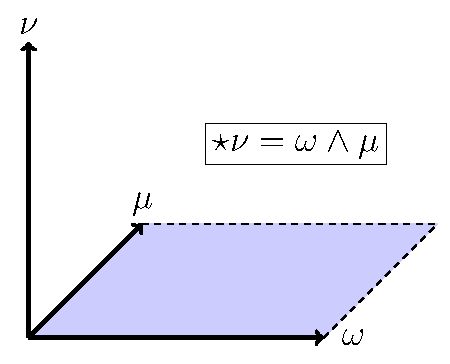
\includegraphics[width=.3\linewidth]{figures/darstellung-hodge.pdf}
\caption{Grafische Darstellung der Funktion des Hodge-Stern-Operators}
\end{figure}

Im Allgemeinen gilt:
 \begin{align}
 g(\omega,\omega) = \prod_{k=1}^{n} g(\sigma^{i},\sigma^{i}) = (-1)^s
 \end{align}
 mit der Signatur $(s,n-s)$, welche die Norm des Vektors festlegt. Die $\sigma^{i}$ sind dabei die orthonormalen Basisvektoren \\
 Für die zweifache Anwendung des Operators gilt: (ohne Herleitung)
 \begin{align}
 \star \star = \star^2 = (-1)^{p(n-p)+s}
 \end{align}
 Wir wollen mit einer etwas anschaulicheren, praktischen Definition arbeiten, welche sich durch kleinere Umformungen aus der abstrakten Definition ergibt. Wir erhalten:
\begin{mybox}{Hodge-Stern-Operator}
\begin{align}
\star(\sigma^1 \w \sigma^2 \w \dots \w \sigma^p) = g(\sigma^1,\sigma^1)\dots g(\sigma^p,\sigma^p) \sigma^{p+1}\w \dots \w \sigma^n
\end{align}
\end{mybox}
Beschränken wir den Operator auf den $\mathbb{R}^3$ verwenden nachfolgend die Notation $\star_s$.
\subsubsection{Anwendungsbeispiel: 4D-Minkowski-Raumzeit}

Wir betrachten den trivialen 4er-Vektor:

\begin{align}
\omega = - \dd t \w \dd x\w \dd y \w \dd z
\end{align}

Wenden wir nun den $\star$-Operator an folgt zum Beispiel:

\begin{itemize}
\begin{align*}
\item \star 1 &= \omega \\
\item \star \omega &= -1 \\
\item  \star \dd t &= - \dd x \w \dd y \w \dd z \\
\item \star \dd x \w \dd y \w \dd z &= - \dd t \\
\item \star\star \omega &= (-1)^{4(4-4)+1} \omega = -\omega \\
\item \dots
\end{align*}
\end{itemize}

Wörtlich gesprochen liefert uns der Hodge-Stern-Operator die duale (n-p)-Form  zur p-Form durch "wedgen" der übrigen Basis-1-Formen, die nicht in der p-Form auftreten, unter Berücksichtigung der Geometrie des Raumes. \\
Dies wollen wir nutzen, um nun die inhomogenen Maxwell-Gleichungen neu auszuformulieren.
	\subsection{inhomogene Maxwell-Gleichungen}
Durch Anwenden des Hodge-Stern-Operators auf $F$ folgt:

\begin{align}
\star F = \star_s E - \star_s B \w \dd t 
\end{align}

und damit:

\begin{align}
\dd \star F &= \star_s \partial_t E  \w \dd t + \dd_s \star_s E - \dd_s \star_s B \w \dd t \notag \\
				&= \dd_s \star_s E + (\star_s \partial_t E - \dd_s \star_s B) \w \dd t 
\end{align}

Vergleicht man dies mit den Maxwell-Gleichungen, fällt auf, dass:

\begin{align}
\star \dd_s \star E &= \varrho \qquad\qquad,\varrho=\text{Ladungsdichte} \\
\star \dd_s\star B - \partial_t E &= j \qquad\qquad ,j=j_x \dd x + j_y \dd y + j_z \dd z
\end{align}

Definiert man den Strom $J=j - \varrho \  \dd t$, lassen sich (17) und (18) in 

\begin{align}
\dd \star F = \star J
\end{align}

zusammenfassen. \\

Insgesamt lässt sich also die gesamte Elektrodynamik auf die beiden gefundenen, äußerst eleganten Gleichungen zurückführen.

\begin{mybox}{Maxwell-Gleichungen}
\begin{align*}
\dd F &= 0 \\
\dd \star F &= \star J
\end{align*}
\end{mybox}

	\subsection{Lagrangian in Differentialformen}

Um den Vortrag abzurunden, kommen wir wieder kurz auf die Lagrange-Beschreibung zurück und zeigen, wie man die Maxwell-Gleichungen in Differentialformen durch einen Lagrangian herleitet. Dazu muss man nun auch den Lagrangian in Differentialformen ausdrücken. \\
Derartige Ausdrücke werden später auch in der Yang-Mills-Theorie un der Chern-Simon-Theorie auftreten. Ihr Vorteil ist, dass sie automatisch alle geforderten Punkte in Kapitel 1 erfüllen, insbesondere die Koordinatenunabhängigkeit. \\

Die Lagrangians setzt man meistens axiomatisch an und zeigt dann, dass sie die gewünschten Gleichungen liefern. Für das elektromagnetische Feld gilt:

\begin{align}
\lagr = - \frac{1}{2} F F + A J,
\end{align}

wobei F, A und J gemäß den obigen Definitionen gegeben sind. Es gelte $F = \d A$. \\

Das zugehörige Wirkungsfunktional ist $\text{I[A]}=\int \lagr$ und sei $A + \varepsilon \cdot \delta A$ das gestörte Eichpotential. \\
Dann folgt aus der Variation der Wirkung: 

\begin{align*}
\frac{d}{d \epsilon} \text{I}[A + \varepsilon \cdot \delta A] &= \frac{d}{d \epsilon} \left( \int - \frac{1}{2} \d(A + \varepsilon \cdot \delta A)  \d(A + \varepsilon \cdot \delta A) + (A + \varepsilon \cdot \delta A) J \right)
&= \int - \frac{1}{2} \left( \d(A + \varepsilon \cdot \delta A)  \d(A + \varepsilon \cdot \delta A) + (A + \varepsilon \cdot \delta A) J \right)
&= .... 

% Hier muss man noch die richtigen Formelzeichen einsetzen...

		
	
% Literatur und Quellen
\thispagestyle{plain}
\nocite{*}
\printbibliography[title=Literaturangaben]


\end{document}
